\chapter{Related Work}\label{chapter:relatedwork}

\section{Dynamic Scene Graph for Video}
The scene graph is a structured representation of a scene that can clearly express the objects, attributes, and relationships between objects in the scene\cite{9661322}. Accompanied by the development of computer vision technology, simply detecting and recognizing objects in images no longer satisfies the researchers, as they would expect some higher level of understanding and reasoning for image vision tasks. In this way, an intuitive idea comes up about adding up the relationship between the detected objects(See example in figure \ref{fig:SGG}). The earliest research could dated back to 2017, when some objects and relations of a given image could be inferred and a scene graph would be produced as a result\cite{xu2017scene}. Other research like Neural Motifs\cite{zellers2018neural} also shows the possibility of predicting the most frequent relation between object pairs with the given labels and object detections. Later in 2018, videos came into discussion, and both spatial and temporal relations would be concerned in the dynamic graph researchers propose to represent\cite{wang2018videos}. Meanwhile, the accuracy of Scene Graph Detection tasks has significantly improved thanks to the application of unbiased SGG\cite{wang2018videos}, fueled by the \textbf{Detection2} \cite{wu2019detectron2}, a library that contains various state-of-the-art detection and segmentation algorithms. In a nutshell, representing videos as dynamic scene graphs including the detection of objects and the relations in between has been realized in the past years. And our work would utilize such technique and extract our driver-oriented dynamic scene graphs for further learning.

\begin{figure}
    \centering
    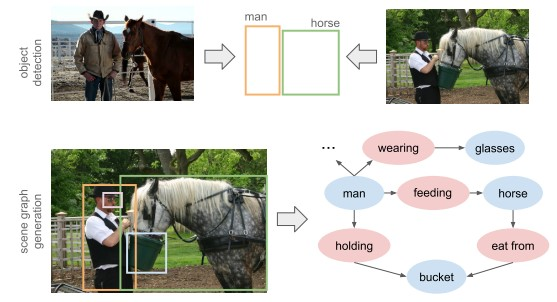
\includegraphics[width=0.8\linewidth]{figures/SGG.jpg}
    \caption{Scene Graph Generation by Iterative Message Passing}
    \label{fig:SGG}
\end{figure}